\subsection{miniWECC-AGC - WIP} 
Ten minute multi-area AGC recovery using optional VTS in PSTv4.
Two different area configurations: One is the same as in \cite{haines2020}, and one made to mimic EIA regions (see Appendix \ref{sec: mw Sys}).
Example allows for comparing VTS to FTS simulation methods.
DC lines are modeled as power injection via load settings.
This power import/export is \textbf{not} included in AGC calculations.
%% MAKE TABLE


%%% MAKE TABLE
%Elapsed Time (FTS):	 1027.2399\\
%Elapsed Time (VTS):	 189.9163\\
%VTS speed up: 5.4089\\

\begin{table}[!ht]
\resizebox{\linewidth}{!}{

	\begin{tabular}{@{} L{1.75cm} 
	R{2cm} R{2cm}  R{2cm} R{1.5cm} R{0.75cm} R{0.75cm} R{1.5cm} R{2cm} R{2cm}@{}} 	
		\toprule % @ signs to remove extra L R space
		\footnotesize % this will affect the table font (makse it 10pt)
		\raggedright % for non justified table text

	&	\multicolumn{3}{c}{Step Size [seconds]}					&		&	\multicolumn{2}{c}{Solutions Per Step}			&		&		&		\\	
\shortstack{PST\\Version}	&	Max.	&	Min.	&	Ave.	&	Total Steps	&	Ave.	&	Max.	&	Total Slns.	&	Sim. Time	&	Speed Up	\\ \midrule	
4.0 - FTS	&	8.33E-3	& 8.33E-3		&	8.33E-3	&	72,001	&	2	&	2	&	144,002	&	782.18	&	1.00	\\	
4.0 - VTS	&	3.32	&	4.07E-06	&	1.18E-01	&	5,094	&	3	&	787	&	15,332	&	151.54	&	5.16	\\	
																				\bottomrule
	\end{tabular}
	}%end resize box
		\caption{PST Version Comparisons of MiniWECC AGC VTS Example.}
		\label{tab: mw AGC}


\end{table}

\noindent VTS is $\approx$5 times faster than FTS and saves $\approx$13x less data.

\begin{figure}[H]
	\centering
	\footnotesize
	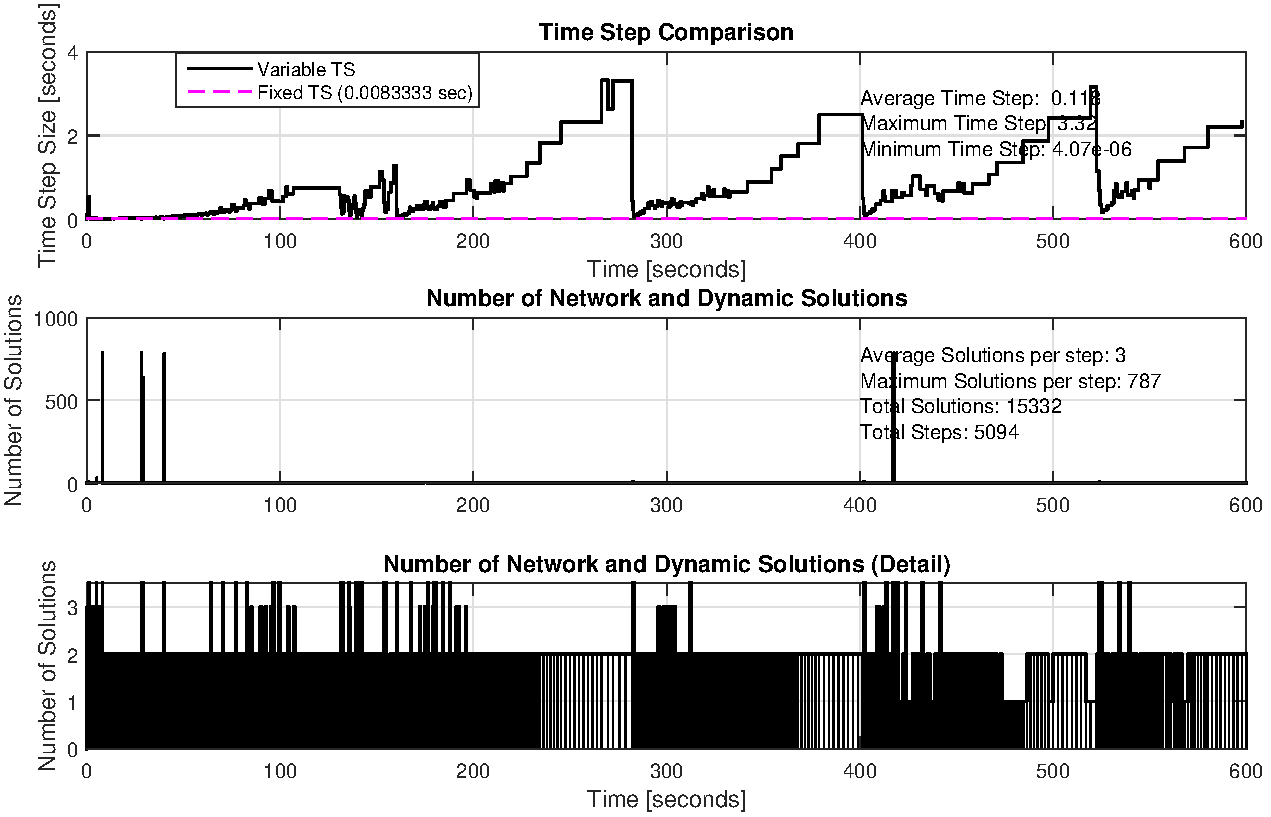
\includegraphics[width=\linewidth]{examples/miniWECC/maAGC-1}
	\caption{MiniWECC AGC recovery FTS vs VTS time step size and solution count.}
	\label{fig: mwAGC steps}
\end{figure}%\vspace{-1 em}


\begin{figure}[H]
	\centering
	\footnotesize
	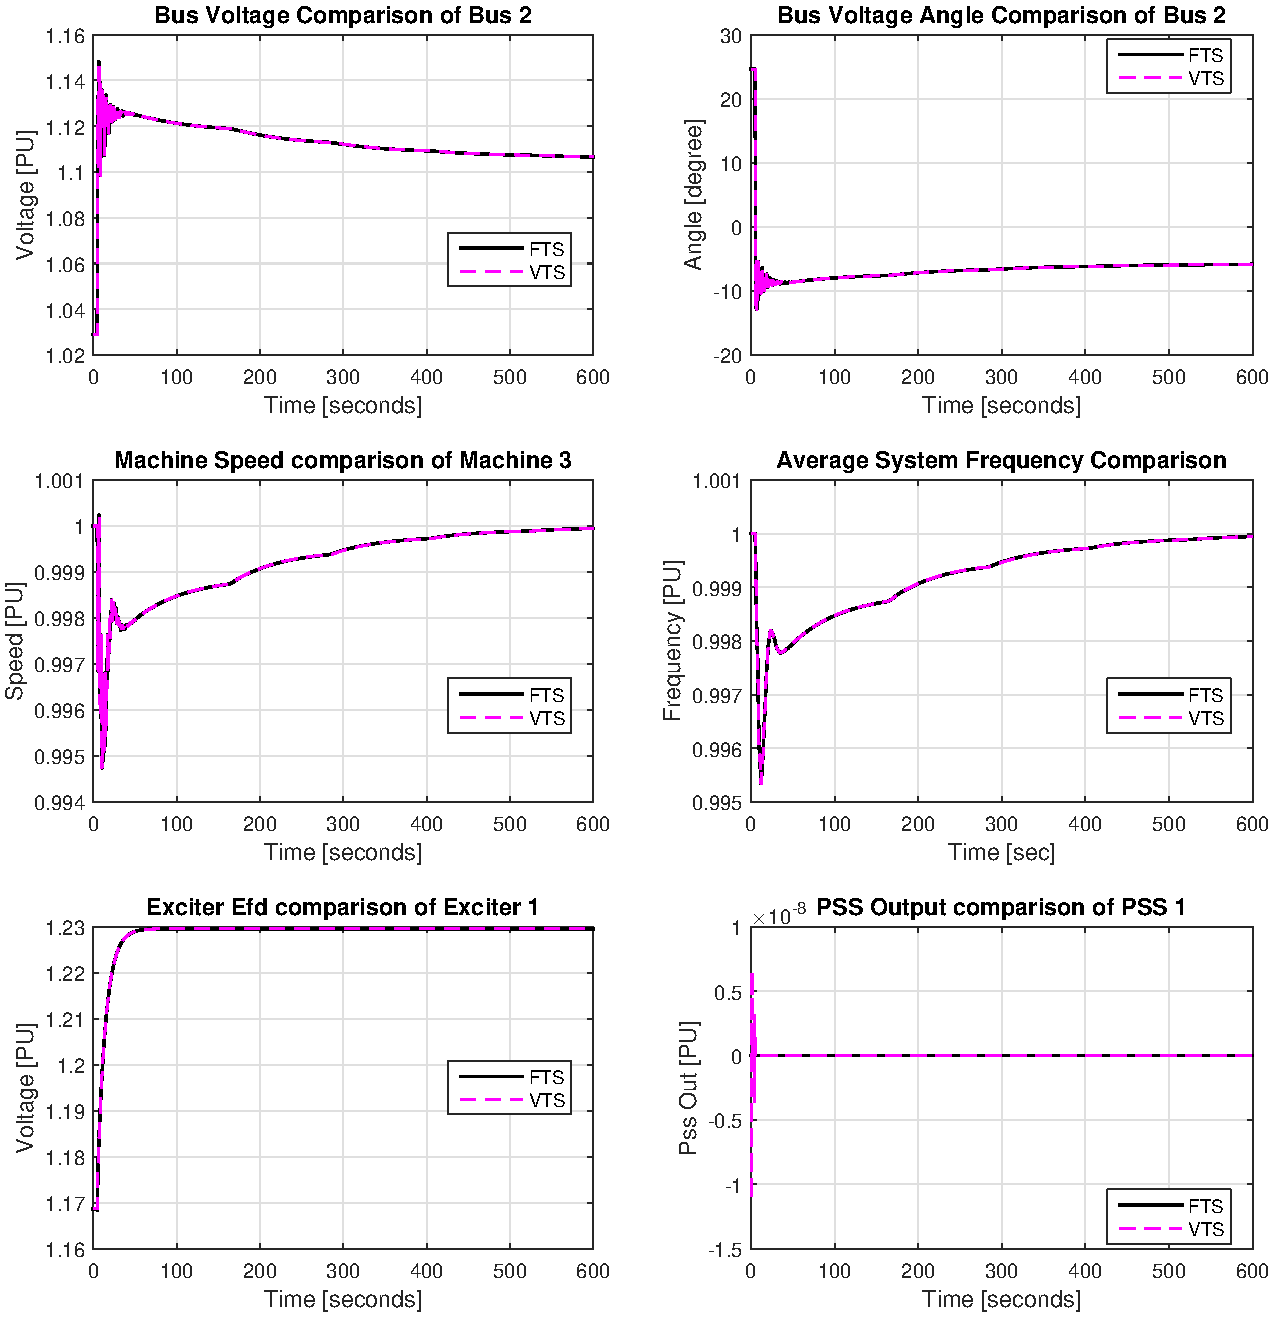
\includegraphics[width=\linewidth]{examples/miniWECC/maAGC-2}
	\caption{MiniWECC AGC recovery FTS vs VTS select comparisons.}
	\label{fig: mwAGC comp}
\end{figure}%\vspace{-1 em}

\begin{figure}[H]
	\centering
	\footnotesize
	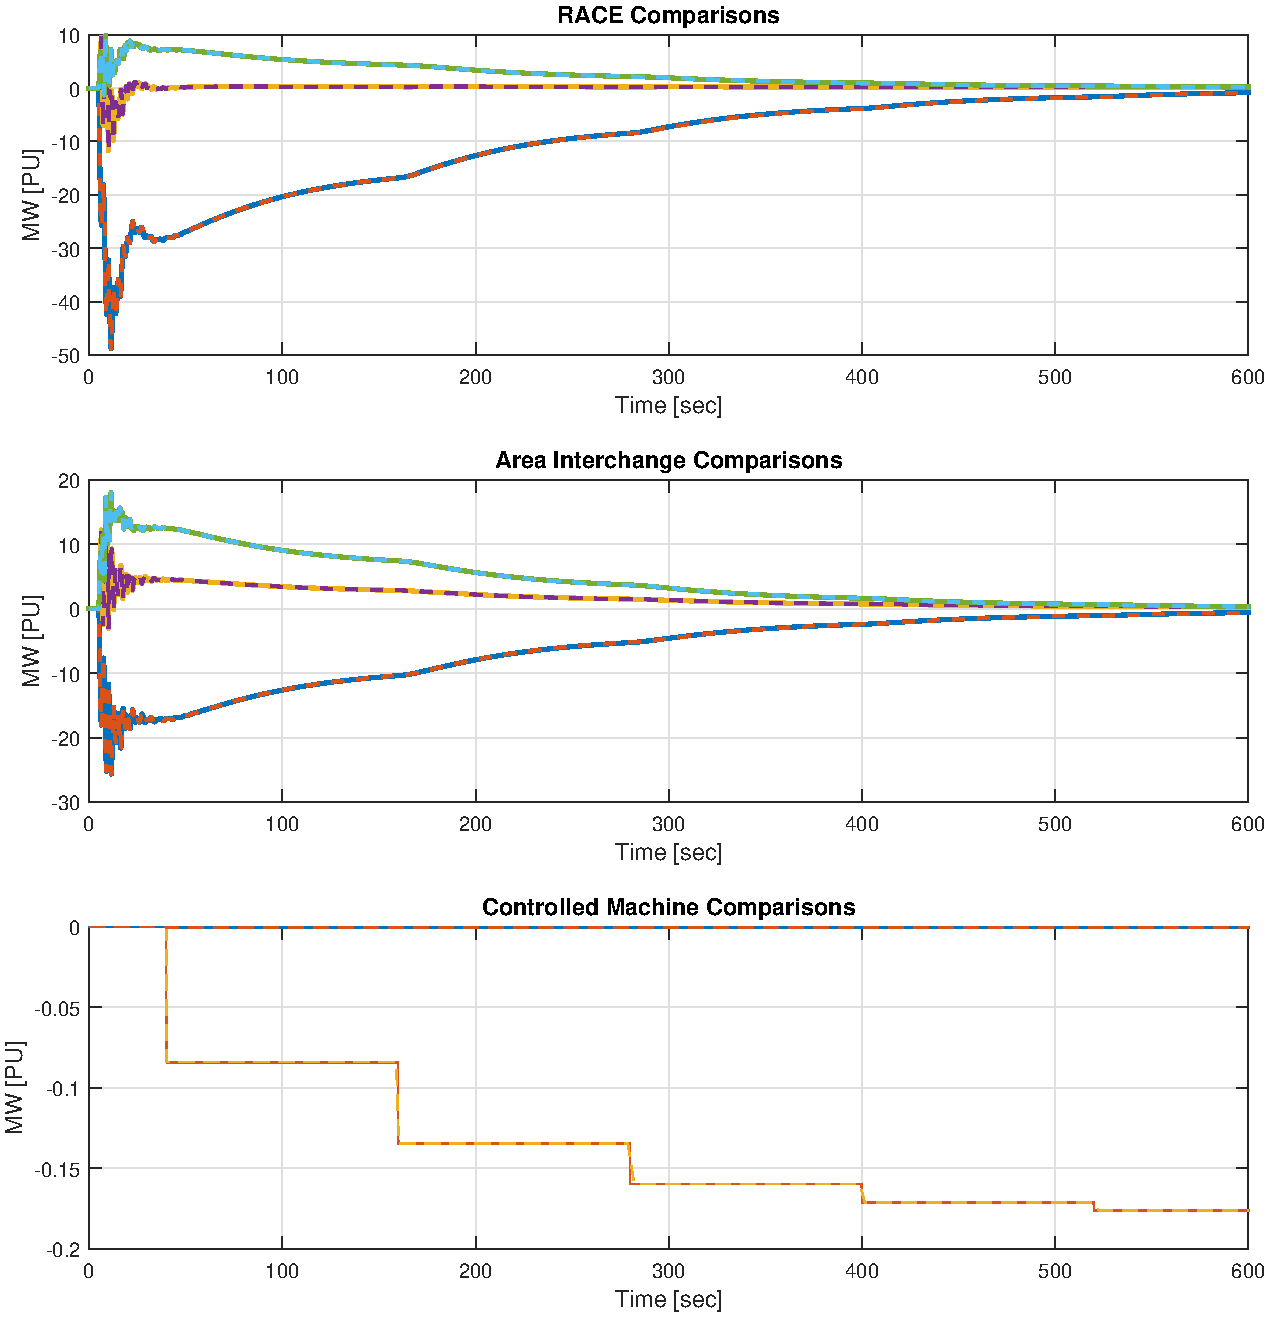
\includegraphics[width=\linewidth]{examples/miniWECC/maAGC-3}
	\caption{MiniWECC AGC recovery FTS vs VTS AGC values.}
	\label{fig: mwAGC agc values}
\end{figure}%\vspace{-1 em}